\section{Introduction}\sloppy
Model training on large and growing datasets is a key data management challenge with significant interest in both industry and academia~\cite{bdas, alexandrov2014stratosphere, crotty2014tupleware, tensor}.
While these frameworks abstract much of the difficult details of distributed Machine Learning (ML), they seldom offer the analyst support in terms of constructing the model itself, such as which features to use or how to represent their data.
The model construction process is still highly iterative, where through trial-and-error, an analyst makes these choices. 
%Eventually she converges onto a model with the desired accuracy.
To further complicate matters, data are often \emph{dirty}, including missing, incorrect, or inconsistent attributes, due to faulty sensors, software, time delays, or hardware.
Thus, although part of the iterative process is tweaking the model paratemers and features, a significant portion involves identifying and cleaning potentially dirty data.  
In our work, we focus on this latter issue. 
While data cleaning is an extensively studied problem, the high dimensionality of many models can amplify even a small amount of erroneous records~\cite{xiaofeature}, and the relative complexity (in comparison to SQL analytics) can make it difficult to trace the consequnces of an error.

To highlight the importance of data cleaning in modern ML pipelines, we have noted the choice of data cleaning algorithm can significantly affect results even when using robust statistical techniques \cite{activecleanarxiv, DBLP:conf/case/MahlerKLSMKPWFAG14}.
For instance, in one fraud prediction example, we found that simply applying Entity Resolution before model training improved true positive detection probabilities from 62\% to 91\%. 
Despite this importance, in theory and in practice, the academic community has decoupled the data cleaning problem from featurization and ML.
This is problematic because many ML techniques often make assumptions about data homogeneity and the consistency of sampling, which can be easily violated if the analyst applies data cleaning in an arbitrary way.

To understand how this may happen, consider an anlyst training a regression model on dirty data. At first, she may not realize that there are outliers and train an initial model directly on the dirty data. 
As she starts to inspect the model and the data, she will soon realize that some records have a large residual error (not predicted accurately). 
Once she confirms that those records are indeed dirty, she has to design rules or scripts to fix or remove the offending records. 
After cleaning, she re-trains the model--iterating until she no longer finds dirty data.
This iterative process is the de facto standard, and is in fact encouraged by the design of the increasingly popular interactive ``notebook" ML development environments (e.g., IPython).
However, this makes the implicit assumption that model training commutes with incremental data cleaning, and the models trained on partially clean data have meaningful predictive value.
This assumption is often incorrect; due to the well-known Simpson's paradox, models trained on a mix of dirty and clean data can have very misleading results even in simple scenarios (Figure \ref{update-arch1}).

\begin{figure}[t]
\centering
 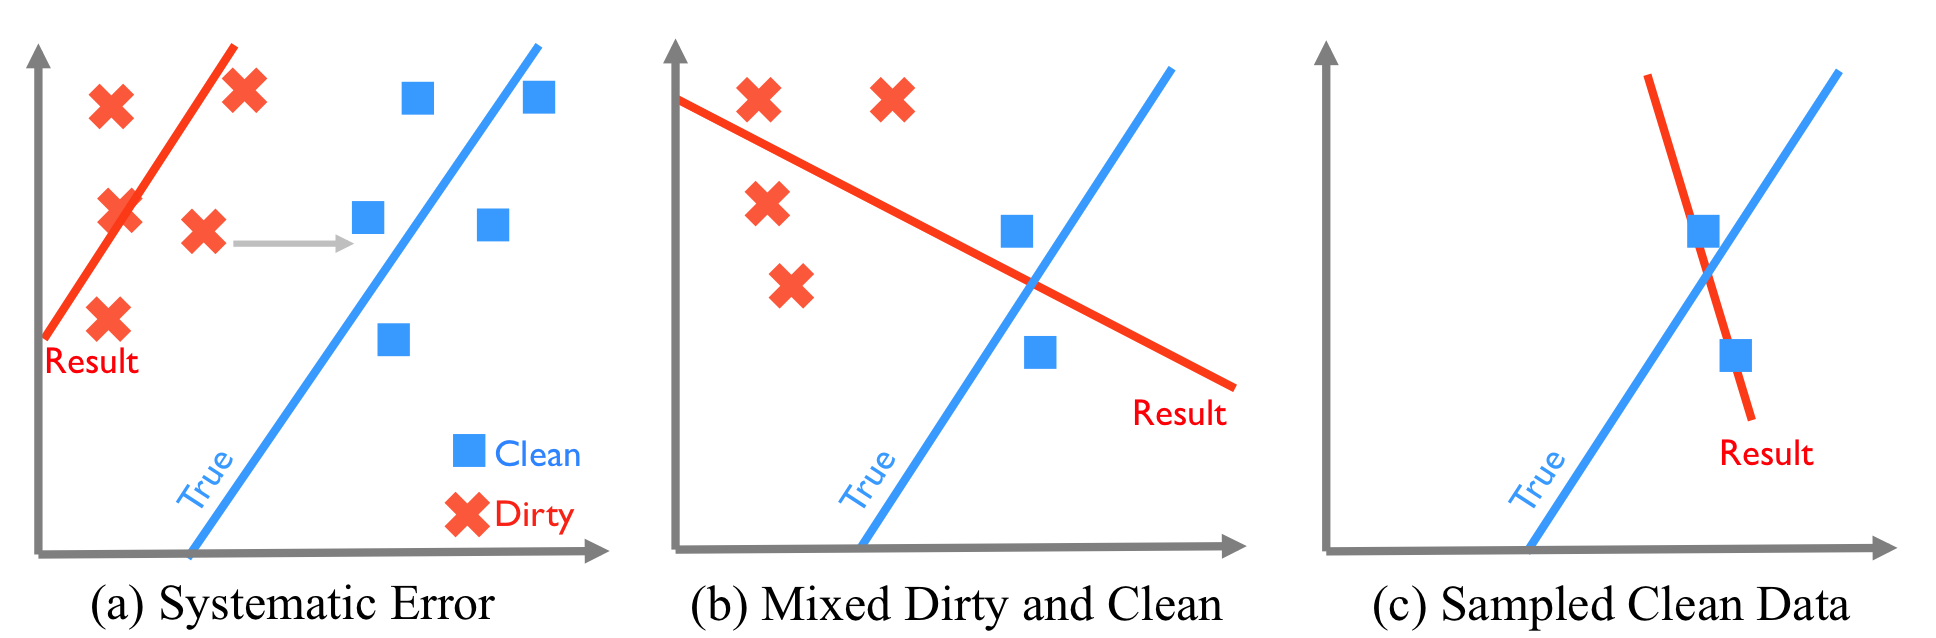
\includegraphics[width=0.8\columnwidth]{figs/update-arch.png}
 \caption{(a) Systematic corruption in one variable (axes) can lead to a shifted model (fitted lines). 
 (b) Mixed dirty and clean data results in a less accurate model than no cleaning.\label{update-arch1}}\vspace{-2em}
\end{figure}

In a parallel trend, the advent of techniques such as Deep Learning and Non-Parametric Bayesian Methods has lead to an explosion in the number of model parameters.
It is now common to use 100,000s of features in image processing processing problems with Convolutional Neural Networks.
Empirically, such feature spaces have facilitated breakthroughs in previously hard classification tasks such as image classification, robot actuation, and speech recognition.
However, the pitfall is that higher dimensional models are harder to debug.
Determining the effects and interaction between dirty data, model error, and counter-intuitive higher dimensional effects can be very challening.

As it stands, there are two key problems in model construction, (1) correctness, and (2) dirty data identification.
We address these two problems in a system called \sys which facilitates interactive training-cleaning iteration in a safe way (with expected monotone convergence guarantees) and automatically selects the most valuable data for the analyst to inspect; even in the complex models popular in modern ML pipelines.
The selection technique applied in \sys uses pointwise gradients to generalize the outlier filtering heuristics to select potentially dirty data even in complex models. 
The analyst initializes an \sys with an ML model, a featurization function, and the base data, and the \sys initially returns the model trained on the dataset.
\sys also returns an set of data sampled from the model that are possibly dirty.
The analyst can apply any value transformations to the data and then prompt the system to iterate. 

Intuitively, \sys prioritizes data cleaning by identifying records, which if cleaned, are likely to change the analyst's model predictions.
\sys applies to a large class of models which can be represented as loss minimization problems solved by gradient descent.
This captures SVMs, Linear Regression, Neural Netorks (Deep Learning), and some types of topic modeling problems such as LDA (for a formal description see \cite{activecleanarxiv}).
In our demonstration, we will show how \sys facilitates debugging complex ML models to understand the effects of dirty data.
The demonstration will consist of a visual interactive interface that will allow the analyst to specify and evaluate a model training pipeline implemented in PySpark~\cite{pyspark}.
The analyst can use the interface to visualize a sample of potentially dirty records and apply data cleaning scripts to different subsets of data.
\sys will correctly incorporate those changes back into the trained model, and allow the analyst to iterate.  
We will present two experimental scenarios where the models are affected by dirty data: 

\begin{example}[Video Segmentation With CNNs]\sloppy
The JHU JIGSAWS Dataset is a corpus of surgical training 120 videos from between 1-5mins long.
These videos are annotated by expert surgeons describing the gestures that occur in the vido. 
Classifying video frames is an important task for segmentation and summarization of future videos.
We would like a classifier that can predict these annotations.
This can be done using Convolutional Neural Networks to featurize frames of the video and then applying a standard classifier like an SVM after the features are extracted.
However, sometimes the annotations are incorrect and \sys can be used to determine when the annotations are incorrect (correspond to the wrong gesture) and inconsistent (multiple gestures simultaneously).
\end{example}

\begin{example}[Topic Modeling With LDA]\sloppy
We have a corpus of reviews from Yelp and we wish to learn a topic model from this dataset.
However, a substantial number of the reviews are spam that typically are soliciting traffic for a fraudulent website.
These spam reviews can affect the distribution of words and affect any models learned from the data.
However, some spam reviews are hard to detect automatically and require human validation.
We can apply \sys to efficiently estimate the topic model without having to validate every review.
\end{example}
 









